%%
%%
%%

\documentclass[cjk,dvipdfm,14pt]{beamer}
\usetheme{Hibi}
\usefonttheme{professionalfonts}
\usepackage{packages}

\title{GHC へのプログラム変換パスの追加}
\author{日比野 啓}
\date{ \today }

%% Lambda式 (Core形式) の書き換えで Haskell のプログラムを変換する

\begin{document}

\lstset{language=Haskell,basicstyle=\small\ttfamily}
  %% commentstyle=\textit,%
  %% classoffset=1,%
  %% keywordstyle=\bfseries,%
  %% frame=tRBl,framesep=5pt,%
  %% showstringspaces=false,%
  %% numbers=left,stepnumber=1,numberstyle=\footnotesize%

\begin{frame}

\maketitle

\end{frame}


\begin{frame}[fragile]
\frametitle{今日の話}

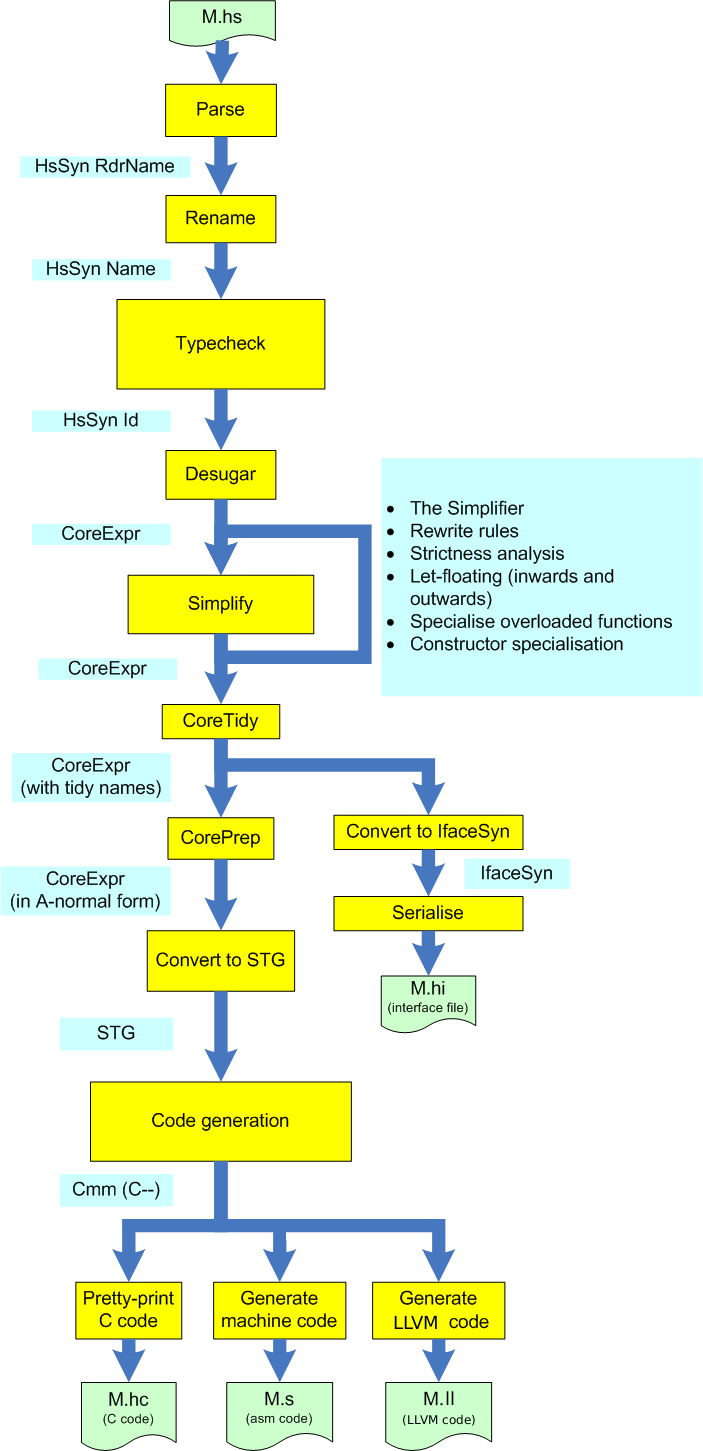
\includegraphics[height=8cm]{./HscPipe2.png}

\end{frame}

\begin{frame}[fragile]
\frametitle{今日の話}

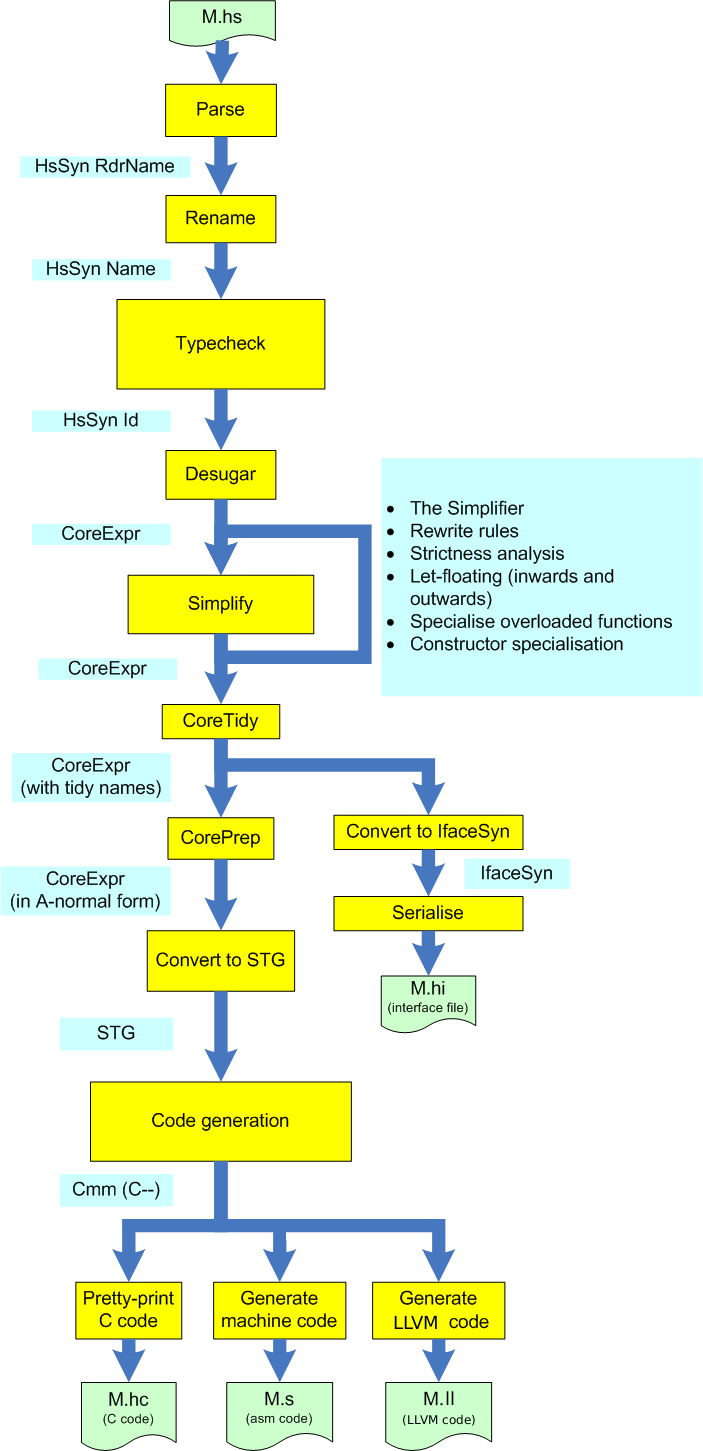
\includegraphics[height=16cm]{./HscPipe2.png}

\end{frame}

%% Haskell から Core へ
%%   ghc -c -ddump-simpl
\begin{frame}[fragile]
\frametitle{HaskellからCoreへ}

\begin{lstlisting}
module Foo (f) where

f :: Int -> Int -> Int
f x y = x * (x + y)
\end{lstlisting}

\hrulefill

Haskell を Core 形式へ変換し、出力するコマンド

\% ghc -c -ddump-simpl Foo.hs

\end{frame}

\begin{frame}[fragile]
\frametitle{Haskell から Core へ}

\begin{lstlisting}
Foo.f :: GHC.Types.Int -> GHC.Types.Int ->
         GHC.Types.Int
[GblId, Arity=2]
Foo.f =
  \ (x_a9H :: GHC.Types.Int)
    (y_a9I :: GHC.Types.Int) ->
    GHC.Num.*
      @ GHC.Types.Int
      GHC.Num.$fNumInt
      x_a9H
      (GHC.Num.+
         @ GHC.Types.Int GHC.Num.$fNumInt
         x_a9H y_a9I)

\end{lstlisting}

\hrulefill

Core は GHC が内部で利用している Lambda式

\end{frame}

\begin{frame}[fragile]
\frametitle{CoreからCoreへ}

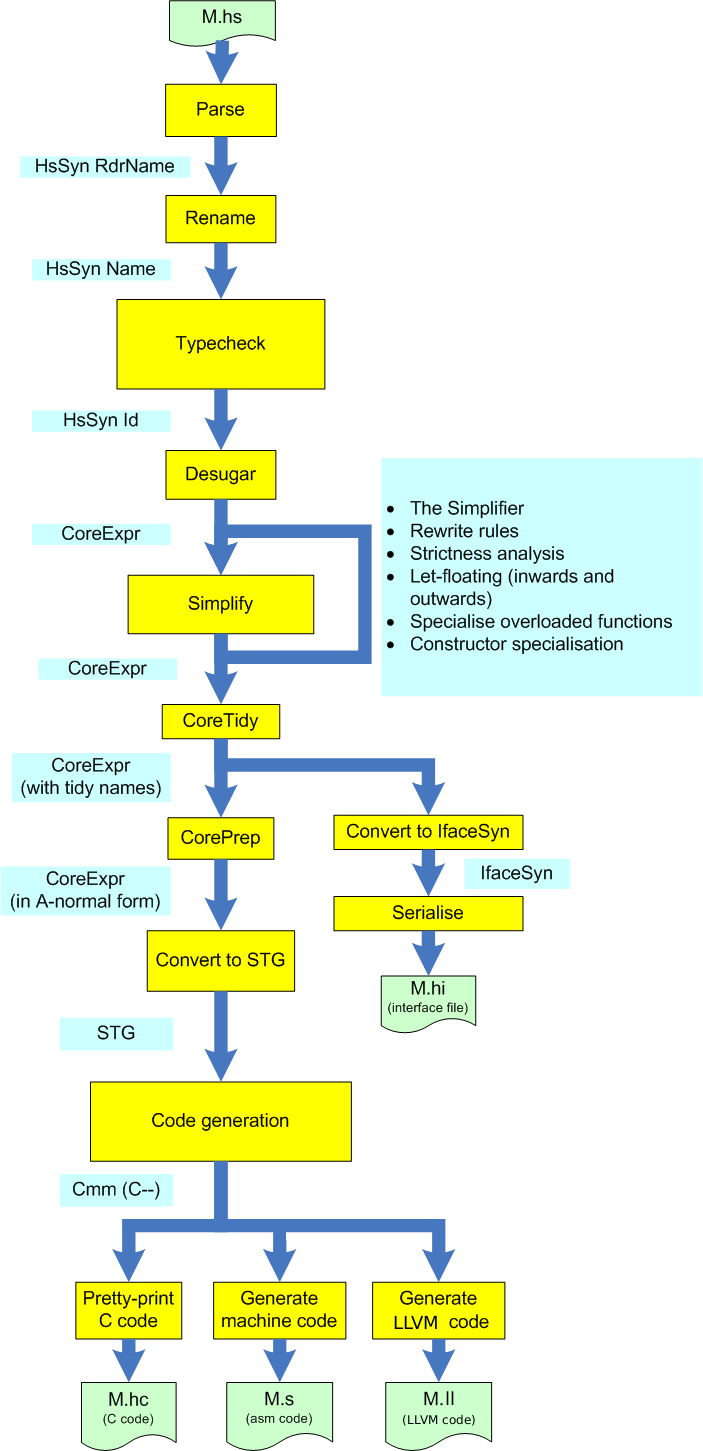
\includegraphics[height=16cm]{./HscPipe2.png}

\end{frame}


%% Core 形式を変換することによってプログラムを書き換える
%%   simplCore

%% 最適化に使ったり


\begin{frame}[fragile]
\frametitle{CoreからCoreへ}

Lambda式を変換すれば、GHCでプログラム変換が書ける。主に最適化のパスを実装する目的で利用されているらしい
\begin{itemize}
\item compiler/simplCore 以下に変換パスの定義
\item compiler/coreSyn 以下にCoreの定義や変換用ライブラリ
\end{itemize}

\end{frame}

\begin{frame}[fragile]
\frametitle{simpl の変換パスの追加}

例えば foo というパスを追加する

\hrulefill

\end{frame}

%% simpl の変換パスの追加 -- 仮に foo というパスを追加する
%%   fooProgram :: CoreProgram -> CoreProgram
%%     CoreSyn.CoreProgram

%%   compiler/simplCore/ 以下
%%        Foo.hs: module Foo (fooProgram) where ...


\begin{frame}[fragile]
\frametitle{simpl の変換パスの追加}

変換パス foo の追加

\hrulefill

compiler/simplCore/Foo.lhs:

\begin{lstlisting}
module Foo (fooProgram) where

import CoreSyn (CoreProgram)

fooProgram :: CoreProgram -> CoreProgram
...
\end{lstlisting}

\end{frame}

\begin{frame}[fragile]
\frametitle{simpl の変換パスの追加}

変換パス foo の追加

\hrulefill

compiler/simplCore/Foo.hs:

\begin{lstlisting}
module Foo (fooProgram) where

import CoreSyn (CoreProgram)

fooProgram :: CoreProgram -> CoreProgram
fooProgram =  id
\end{lstlisting}

\end{frame}


%%   compiler/simplCore/ 以下
%%   CoreMonad.CoreToDo (CoreFoo)

\begin{frame}[fragile]
\frametitle{simpl の変換パスの追加}

変換パス foo の追加

\hrulefill

compiler/simplCore/CoreMonad.lhs

\begin{lstlisting}

data CoreToDo ...

  ...
  | CoreFoo
  ...
\end{lstlisting}

\end{frame}

%% compiler/main/ 以下
%%   DynFlags.DynFlag (Opt_Foo)

\begin{frame}[fragile]
\frametitle{simpl の変換パスの追加}

変換パス foo の追加

\hrulefill

compiler/man/DynFlags.hs

\begin{lstlisting}
data DynFlag
   ...
   -- optimisation opts
   ...
   | Opt_Foo
   ...
fFlags = [
  ...
  ( "foo",  Opt_Foo, nop ),
  ...  ]
\end{lstlisting}

\end{frame}


%% compiler/coreSyn/ 以下
%%   SimpleCore.getCoreToDo
%%     ...
%%     foo           = dopt Opt_Foo
%%     ...
%%     runWhen foo CoreFoo
%%   SimpleCore.doCorePass CoreFoo  = {-# SCC "Foo" #-}
%%                                    doPass fooProgram

\begin{frame}[fragile]
\frametitle{simpl の変換パスの追加}

変換パス foo の追加

\hrulefill

compiler/coreSyn/SimpleCore.lhs

\begin{lstlisting}
...
getCoreToDo
  ...
  where
    ...
    strictness = dopt Opt_Strictness  dflags
    ...
    foo        = dopt Opt_foo         dflags
    ...
\end{lstlisting}

\end{frame}

\begin{frame}[fragile]
\frametitle{simpl の変換パスの追加}

変換パス foo の追加

\hrulefill

compiler/coreSyn/SimpleCore.lhs

\begin{lstlisting}
...
getCoreToDo
  ...
  [ ...
    runWhen strictness ... ,
    ...
    runWhen foo CoreFoo,
    ...
  ]
\end{lstlisting}

\end{frame}

\begin{frame}[fragile]
\frametitle{simpl の変換パスの追加}

変換パス foo の追加

\hrulefill

compiler/coreSyn/SimpleCore.lhs

\begin{lstlisting}
import Foo (fooProgram)
...
doCorePass :: CoreToDo -> ...
...
doCorePass CoreFoo = doPass fooProgram
...
\end{lstlisting}

\end{frame}

\begin{frame}[fragile]
\frametitle{simpl の変換パスの追加}

変換パス foo の追加

\hrulefill

\begin{itemize}
\item ここまでの変更で、コンパイラに -O1 -ffoo スイッチを与えれば、
Foo (fooProgram) でプログラムが変換されるようになっているはず。
\item あとは Foo.hs を実装すればよい
\end{itemize}

\end{frame}

%% 利用できるライブラリ
%%   base, containers ...
%%   TrieMap.CoreMap

\begin{frame}[fragile]
\frametitle{利用できるライブラリ}

外部ライブラリと同じものでは

\begin{itemize}
\item ex. -package Cabal-1.14.0 -package array-0.4.0.0 -package base-4.5.0.0
-package bin-package-db-0.0.0.0 -package bytestring-0.9.2.1
-package containers-0.4.2.1 -package directory-1.1.0.2 -package filepath-1.3.0.0
-package hoopl-3.8.7.3 -package hpc-0.5.1.1 -package old-time-1.1.0.0
-package process-1.1.0.1 -package unix-2.5.1.0
\end{itemize}

\end{frame}


\begin{frame}[fragile]
\frametitle{利用できるライブラリ}

コンパイラ内部だと
\begin{itemize}
\item TrieMap(CoreMap)
 \begin{itemize}
 \item CoreExpr を key とした Map
 \end{itemize}
\item CoreSubst(Subst)
 \begin{itemize}
 \item Core Syntax を置換するためのデータ構造
 \end{itemize}
\end{itemize}
\end{frame}

%% CSE (Common SubExpression Elimination)

%%  PRE (Partial redundancy elimination) とも
%%  式の字面で判断して共通式を除去

\begin{frame}[fragile]
\frametitle{実装されている最適化パスの例}

CSE (Common SubExpression Elimination)

\begin{itemize}
\item -O1 -fcse
\item PRE (Partial redundancy elimination) とも
\item 式の字面で判断して共通式を除去
\end{itemize}


%%  x = p + q
%%  y = p + q
%%    ↓
%%  x = p + q   -- Map  p + q => x
%%  y = p + q   -- 置き換え対象
%%    ↓
%%  x = p + q   -- Map  p + q => x
%%  y = x

\end{frame}

\begin{frame}[fragile]
\frametitle{CSE}

\begin{lstlisting}
  x = p + q
  y = p + q
  -- ↓
  x = p + q   -- Map  p + q => x
  y = p + q   -- 置き換え対象
  -- ↓
  x = p + q   -- Map  p + q => x
  y = x
\end{lstlisting}

\end{frame}


%%  r = p
%%  s = q
%%  x = p + q
%%  y = r + s
%%  -- ↓
%%  r = p
%%  s = q
%%  x = p + q   -- Map  p + q => x
%%  y = r + s   -- Map  r + s => y
%%              -- 置き換え対象が無い

\begin{frame}[fragile]
\frametitle{CSE}

\begin{lstlisting}
  r = p
  s = q
  x = p + q
  y = r + s
  -- ↓
  r = p
  s = q
  x = p + q   -- Map  p + q => x
  y = r + s   -- Map  r + s => y
              -- 置き換え対象が無い
\end{lstlisting}

\end{frame}


%%   用語 SSA (Static single assignment)


%% GVN (Global value numbering)
%%   式が生成する値ごとに異なる番号を付けていき、同じ番号の付いた式を除去する

\begin{frame}[fragile]
\frametitle{自分でも最適化パスを追加してみました}

GVN (Global value numbering)

\begin{itemize}
\item 式が生成する値ごとに異なる番号を付けていき、同じ番号の付いた式を除去する
\end{itemize}

\end{frame}

%%  -- p, q は自由変数
%%  r = p
%%  s = q
%%  x = p + q
%%  y = r + s
%%  z = x * y
%%


\begin{frame}[fragile]
\frametitle{GVN}

\begin{lstlisting}
  -- p, q は自由変数
  r = p
  s = q
  x = p + q
  y = r + s
  z = x * y
\end{lstlisting}

\end{frame}

%%  z = x * y -- 略
%%            -- hash [r + s] = hplus [hash[r], hash[+], hash[s]]
%%                            = hplus [      1,       2,       3] -- p => 1, (+) => 2, q => 3,
%%                                                                -- r => 1, s => 3
%%                            = 123 -- この例では例えば 123 になったとしておく
%%  y = r + s -- y => 123
%%  x = p + q -- x => 123
%%  s = q     -- s => 2, q => 2
%%  r = p     -- r => 1, r => 1

\begin{frame}[fragile]
\frametitle{GVN}

\begin{lstlisting}
  z = x * y -- 略
  -- hash[r + s] = hplus[hash[r],
  --                     hash[+],
  --                     hash[s]]
  --             -- p => 1, (+) => 2, q => 3,
  --             -- r => 1, s => 3
  --             = hplus[ 1, 2, 3]
  --             = 123
  --  この例では例えば 123 になったとしておく
  y = r + s -- y => 123
  x = p + q -- x => 123
  s = q     -- s => 2, q => 2
  r = p     -- r => 1, r => 1
\end{lstlisting}

\end{frame}

%%  1:   r ==> p
%%  2:   s ==> q
%%  123: y ==> x
%%
%%  r = p     -- 除去可能
%%  s = q     -- 除去可能
%%  x = p + q
%%  y = p + q -- 除去可能
%%  z = x * x

\begin{frame}[fragile]
\frametitle{GVN}

\begin{lstlisting}
  y = r + s -- y => 123
  x = p + q -- x => 123
  s = q     -- s => 2, q => 2
  r = p     -- r => 1, r => 1

  -- 1:   r ==> p
  -- 2:   s ==> q
  -- 123: y ==> x
\end{lstlisting}

\end{frame}

\begin{frame}[fragile]
\frametitle{GVN}

\begin{lstlisting}
  -- 1:   r ==> p
  -- 2:   s ==> q
  -- 123: y ==> x

  r = p     -- 変化なし      -- 除去可能
  s = q     -- 変化なし      -- 除去可能
  x = p + q -- 変化なし
  y = p + q -- <-- y = r + s -- 除去可能
  z = x * x -- <-- z = x * y
\end{lstlisting}

\end{frame}


\begin{frame}[fragile]
\frametitle{デモ}

{ \Huge デモ }

\end{frame}

\begin{frame}[fragile]
\frametitle{まとめ}

\begin{itemize}
\item Lambda式 Core の変換でプログラム変換を実装できる
\item ライブラリも結構使えるので書きやすい
\item GVN を実装してみた。が不完全なのでもうちょっとがんばりたい
\item Compiler plugin化もしてみたい
\end{itemize}

\end{frame}

\end{document}


%% \begin{frame}

%% \frametitle{Agenda}

%% \begin{itemize}
%% \item Cabal
%% %%\item Cabal
%% \item Debian
%% \end{itemize}

%% \end{frame}

%% \begin{frame}

%% \frametitle{Agenda}

%% \begin{itemize}
%% \item {\color{red} Cabal}
%% %% \item Cabal
%% \item Debian
%% \end{itemize}

%% \end{frame}
